% !TEX encoding = UTF-8 Unicode
\documentclass[a4paper]{article}

\usepackage[utf8]{inputenc}
\usepackage{erk}
\usepackage{cite}
\usepackage{tikz}
\usepackage{times}
\usepackage{graphicx}
\usepackage{graphicx}
%\usepackage{caption}
\usepackage{subcaption}
\usepackage[top=22.5mm, bottom=22.5mm, left=22.5mm, right=22.5mm]{geometry}
\usetikzlibrary{shapes, fit, arrows, calc, positioning}

\tikzstyle{block} = [draw, rectangle, minimum width = 0.75cm, minimum height = 0.75cm]
\tikzstyle{sum} = [draw, circle, minimum size=.5cm, node distance=1.75cm]
\tikzstyle{input} = [coordinate]
\tikzstyle{output} = [coordinate]
\tikzstyle{support} = [coordinate]
% USER DEFINED MACROS
\newcommand{\matlab}{MATLAB\textsuperscript{\textregistered}}
\newcommand{\simulink}{SIMULINK\textsuperscript{\textregistered}}
\newcommand{\matsim}{MATLAB\textsuperscript{\textregistered} SIMULINK\textsuperscript{\textregistered}}
\newcommand{\thom}{$\textbf{T}^i_{i+1}$}
\newcommand{\Lagrt}{\mathcal{T}}
\newcommand{\Lagrl}{\mathcal{L}}
\newcommand{\Lagru}{\mathcal{U}}
\usepackage[slovene,english]{babel}

% local definitions
\def\footnotemark{}%  to avoid footnote on cover page

\begin{document}
%make title
\title{UDP-ARCNET strežnik za krmiljenje robota PA-10}

\author{Timotej Gašpar$^{1}$, Leon Žlajpah$^{2}$} % use ^1, ^2 for author(s) from different institutions

\affiliation{$^{1}$Fakulteta za elektrotehniko\\ 
$^{2}$Institut Jožef Štefan}

\email{E-pošta: timotej.gaspar@gmail.com}

\maketitle

%\thispagestyle{empty}

\begin{abstract}{UDP-ARCNET server for control of PA-10 robot}

Servo motor controller of industrial robots usually allows the users very limited control. Manufacturers hardly provide detailed information on the low level motor control. In spate of that, Mitsubishi Portable Intelligent Arm PA-10 comes with a good documentation on the servo driver. It allows the user to know all the parameters of servo motor regulation. The servo also allows the user to control each motor separately in velocity or torque mode opening various options in terms of control. The servo controller has an ARCNET module for communication in the ARCNET network, through witch the user can access and set the regulation parameters and motor control.

When designing end point robot control, the faster the regulation frequency is, the better performance one can achieve. 

A UDP-ARCNET server was built as a man in the middle for servo controller communication with the wish to achieve high control frequencies. The server allows control frequencies up to 500 Hz. It was build on Linux operating system in the low level programming language C.

The server allows the users to control the robot via custom programs that allow UDP communication. For evaluation purposes of the server, admittance control is implemented and tested.

\end{abstract}


\selectlanguage{slovene}

\section{Uvod}

Raziskovalne institucije, ki raziskujejo algoritme vodenja robotov imajo izbiro ali konstruirajo svojega robota in s tem poznajo vse njegove dinamične lastnosti ter točno vedo kako se krmilijo motorji ali pa se odločijo za uporabo industrijskega robota. V slednjem primeru pa so prepuščeni podatkom, ki jih dobijo od proizvajalca. Tem pa običajno ni v interesu podati vseh podatkov glede konstrukcije robota ter zgradbe servo krmilnika zaradi bojazni, da bodo prišli v roke konkurenčnim podjetjem.

Robotski mehanizem Mitsubishi Portable Inteligent Arm PA-10 je iz tega razloga idealen za raziskovalne namene. Poleg že tako bogate dokumentacije in odprtosti krmilnika ga odlikuje še razširjenost po raziskovalnih institucija, kar pomeni, da so njegovi dinamični parametri zelo dobro poznani. Dodatno pa je proizvajalec podal dokumentacijo v kateri podrobno opiše delovanje krmilnika servo motorjev. 


\section{Robotski mehanizem PA-10}

Podjetje Mitsubishi Heavy Industries je leta 1992 izdelalo prvega katalogiranega industrijskega redundantnega robota \cite{mhi_pa10}. Podjetje je robota poimenovalo Portable General-purpose Intelligent Arm PA-10, krajše PA-10. Gre za serijskega robota s sedmimi stopnjami prostosti. Prvi trije sklepi so označeni kot ramenski sklepi (shoulder), S1, S2, S3

Masa robotske roke PA-10 je 36 kg in ima nosilnost 10 kg. Servo motorji v sklepih se napajajo preko izmenične napetosti. Prenosi med v sklepih so realizirani z harmoničnimi gonili. Baza robota da se lahko pritrdi v katerokoli lego. To pomeni, da se ga lahko fiksira bodisi na tla, na steno ali na strop. Robota PA-10 odlikuje relativno lahka konstrukcija, enostavno rokovanje ter odprtost njegovega krmilnika. Prav ti razlogi so povod, da je mnogo instituciji vzelo tega robota kot eksperimentalni sistem za razvijanje raznih algoritmov vodenja (\cite{voung_pa10}, \cite{aalst_pa10}, \cite{rodrigo_pa10},\cite{petric_nevronska}).

\section{UDP-ARCNET strežnik}

Krmilnik omogoča vodenje servo motorjev bodisi preko referenčne hitrosti ali referenčnega navora. V krmilniku je vgrajen ARCNET vmesnik, ki omogoča priklop krmilnika v ARCNET omrežje. Na ta način je omogočena komunikacija s krmilnikom \cite{pa10-manual}.

Z uspešnim vodenjem robota brez taktilne povratne zanke je mogoče izvesti mnogo različnih nalog. S poznavanjem vseh dinamičnih parametrov je v teoriji mogoče izračunati sile, ki delujejo na vrh robota $\textbf{h}_o$. V praksi se izkaže, da te parametre ni vedno mogoče dovolj natančno definirati. Iz teh razlogov se vgradi senzor sil in navorov med vrhom robota ter prijemalom (\cite{almassri_pressure_sensor}, \cite{mihelj_vodenje}, \cite{eppinger_force_dynamics}). Pri izvedbi tega dela se je uporabili senzor sil in navorov JR3. Želja po združitvi vodenja robota in merjenja sil je privedla do tega, da smo avtorji naredili  strežnik, ki to omogoča. Dodaten razlog je bil to, da prejšnja programska oprema za komunikacijo s servo krmilnikom, ni zadoščala časovnemu kriteriju delovanja s frekvenco 500 Hz.

\subsection{Krmilnik servo motorjev robota} \label{sec:servo-drive}

V ohišju servo krmilnika so vgrajeni štirje krmilniki servo motorjev. Vsak servo krmilnik krmili dva servo motorja, razen enega. Krmilniki omogočajo vodenje motorjev na dva načina. Prvi način je navorno, drugi pa hitrostno. Različna vodenja sta v krmilnikih drugače realizirana. Navorno vodenje je realizirano z analognim P regulatorjem toka, hitrostna regulacija pa je realizirana z digitalnim PI regulatorjem s frekvenco približno 1500 Hz.

Krmilnik vsebuje dva pomnilnika. Delovni pomnilnik (RAM) in nastavitveni pomnilnik (EEPROM). V EEPROM tabeli so zapisani razni parametri za nastavitve in vodenje servo krmilnikov. Ob vžigu krmilnika se parametri naložijo iz EEPROM tabele v RAM. Med temi parametri so tudi ojačanje proporcionalnega ter integracijskega dela regulatorja, omejitve posameznih stopenj, razmerje prenosa zobnikov, itd.

\subsection{ARCNET vmesnik}\label{sec:arc_drive}

Referenčne navore in hitrosti se na krmilniku nastavlja na preko zunanjega vmesnika, ki je povezan na enako ARCNET omrežje kot servo krmilnik. ARCNET je omrežje, ki vključuje podatkovni in fizični nivo po OSI modelu, komunikacija po omrežju pa je serijska in paketno zastavljena. Njegova prednost pred Ethernet omrežjem je velika stopnja determinističnosti \cite{arc_tutorial}. Krmilnik ima dva priključka za optična 
vodila, vhod (Rx) ter izhod (Tx). Zgornja meja hitrosti komunikacije za robota PA-10 je 5 Mb/s \cite{pa10-manual}.

ARCNET modul dodatno vsebuje logiko za preklapljanje med različnimi stanji. Med stanji preklapljamo s pošiljanjem ustrezne črke v paketu. Različna stanja pa so:

\begin{itemize}
	\item Izpis EEPROM tabele,
	\item Vpis v EEPROM tabelo,
	\item Vpis v RAM tabelo,
	\item Kopiranje iz RAM v EEPROM tabelo,
	\item Postavitev kotov na ničelno vrednost,	
	\item Sporstitev zavor,
	\item Vodenje sklepov,
	\item Čakanje
\end{itemize}

Ko višje nivojski vmesnik ne pošilja nobenih ukazov je ARCNET vmesnik v čakanju. V tem stanju čaka na primerno sestavljen paket.

\subsection{Senzor sile in navorov - JR3}

Na vrh robota je pritrjen senzor sil in navorov JR3. Senzor omogoča merjenje sil in navorov v X, Y in Z oseh. Uporovni lističi porazdeljeni po notranjosti senzorja se deformirajo pod vplivom sile. Upornost na uporovnih lističih spremeni proporcionalno s silo, ki deluje na senzor. Sprememba upornosti se izmeri posredno preko spremembe napetosti na AD-pretvorniku, ki je vgrajen v sam senzor. 

Napetost se pretvori v silo 

\begin{equation}
\textbf{h}_{JR3} = \textbf{K} \mathbf{\omega}_u,
\end{equation}
kjer je \textbf{K} kalibracijska matrika, $\mathbf{\omega}_u$ vektor napetosti na AD-pretvorniku, $\textbf{h}_{JR3}$ pa vektor sil.


Senzor se priključi preko 6 ali 8 žičnega kabla na računalniško kartico, ki je bodisi na ISA ali PCI vodilu. Kabel serijsko pošilja podatke o izmerjenih silah na kartico. Kartica vsebuje vezje za digitalno obdelavo signalov. V dokumentaciji kartice \cite{jr3_doc_inst} so opisani trije nizkoprepustni filtri z različnimi mejnimi frekvencami. V tem delu se je uporabilo filter z mejno frekvenco 500 Hz.

Na računalniku, ki se je uporabljal za to delo, je nameščena kartica na vodilu ISA. Ker je standard starejši, je podjetje prenehalo s podporo tega standarda. Kot posledica tega so avtorji tega dela razvili svojo programsko opremo za komunikacijo z notranjimi registri kartice.

\subsection{Strežnik} \label{sec:streznik}

Proizvajalec Mitsubishi Heavy Industries je za upravljanje in programiranje robota pripravil posebno programsko opremo. Iz dokumentacije je razvidno kaj je vse njihova programska oprema omogočala. Težava pa je, da omenjena programska oprema ni več dostopna. Proizvajalec je s prodajo robotov PA-10 prenehal v letu 2009, s podporo pa v marcu 2014 (vir: osebno dopisovanje s proizvajalcem). Iz tega razloga je nastala potreba, po lastnem programu, ki bi lahko komuniciral s servo krmilnikom.

Pred začetkom izdelave lastnega programskega orodja se je definiralo dve zahtevi. Prva je bila, da program deluje kar se le da hitro in kar se le da v realnem času. To izhaja iz vidika stabilnosti vodenja. Avtor v \cite{mihelj_hapt} namreč navaja, da vzorčni čas močno vpliva na stabilnost vodenja robota v kontaktu z okolico. Večja kot je vzorčna frekvenca večja je lahko togost okolice s katero je robot v kontaktu.

Druga zahteva pa je bila enostavna uporaba. Želeli smo, da uporaba programske opreme, ki jo naredimo, zahteva čim manj predznanja o komunikacijskih protokolih po ARCNET mreži. Hkrati pa mora program omogočati neko mero svobode pri realizaciji visoko nivojskega vodenja.

Dodatno se je kasneje pojavila še želja, da bi programska oprema omogočala tudi posredovanje meritev izvedenih na senzorju sile JR3. Tako bi nastal nek program, ki bi komuniciral tako s servo kontrolerjem kot s ISA kartico za senzor sile JR3.

Naštete zahteve so privedle do izbire primernega operacijskega sistema in programskega jezika. Tako je bil razvit strežnik v programskem jeziku C na operacijskem sistemu Linux. Strežnik deluje kot posrednik med dvema različnima omrežjema, ARCNET in UDP.  V nadaljevanju bo opisana zgradba tega strežnika, delovanje ter uporaba.

\section{Admitančno vodenje}

Vodenje robota preko vhodnih hitrostih v sklepih je relativno enostaven problem saj PI regulator v krmilniku poskrbi, da se vsak sklep vrti s hitrostjo čimbolj podobno referenčni. Iz tega vidika je prednost ta, da ne glede na konfiguracijo ter obremenitev robota, bo regulator vedno poskrbel čim boljše sledenje referenci. Vplivi gravitacije se kompenzirajo z integrirnim členom v regulatorju. V nadaljevanju bo opisano vodenje motorjev robota v želeno lego oziroma vodenje robota v notranjih koordinatah. Nato pa se bo iz tega še izpeljalo vodenje v zunanjih koordinatah.


\subsection{Vodenje v notranjih koordinatah} \label{sec:admit_inner}

Krmilnik servo motorjev nam v vsakem danem trenutku vrača trenuten kot v sklepu. Ker ima PI regulator visoka ojačanja ter visoko frekvenco, bomo za namene poenostavitve aproksimirali motor kot integrator $\frac{1}{s}$. Naj bo referenčni kot v sklepih označen kot $\textbf{q}_{ref}$ in naj bo dejanski kot označen kot $\textbf{q}$. Razlika med njima je napaka v kotu 

\begin{equation}
\tilde{\textbf{q}} = \textbf{q}_{ref} - \textbf{q}.
\end{equation}
S preprostim P regulatorjem lahko kote v sklepu robota vodimo s povratno zanko. Ojačanje regulatorja bo označeno s $\textbf{K}_p$ in je diagonalna saj ima vsak sklep svoje ojačanje neodvisno od ostalih. S povečevanjem ojačanja regulatorja \textbf{K} vplivamo na dinamiko odziva \cite{zupancic_tr}.

\begin{equation} \label{eq:p_reg_q}
\textbf{u} = \textbf{K}_p  \tilde{\textbf{q}}.
\end{equation}


Za boljšo stabilnosti vnesemo še signal dušenja $\textbf{K}_d \dot{\mathbf{q}}$. Matrika $\textbf{K}_d$ je tako kot $\textbf{K}_p$ diagonalna. Regulirni signal sedaj zapišemo kot

\begin{equation} \label{eq:pd_reg_q}
\textbf{u} = \textbf{K}_p \tilde{\mathbf{q}} - \textbf{K}_d \dot{\mathbf{q}}.
\end{equation}

Vodenje robota po notranjih koordinatah je sredstvo za realizacijo vodenja v zunanjih koordinatah saj se samo po sebi redko uporablja.

\subsection{Vodenje v zunajih koordinatah} \label{sec:admit_out}

Naj bo $\textbf{x}_{ref}$ vektor referenčne lege vrha robota in naj bo $\textbf{x}$ trenutna lega vrha robota. Napaka je tako

\begin{equation} \label{eq:xerr}
\tilde{\textbf{x}} = \textbf{x}_{ref}  - \textbf{x}
\end{equation}

Enačba direktne kinematike nam govori o odnosu med hitrostjo vrha robota ter hitrostjo v sklepih robota

\begin{equation} \label{eq:qtox}
\dot{\textbf{x}} = \textbf{J}(\textbf{q})  \dot{\textbf{q}}.
\end{equation}

To enačbo je mogoče razumeti tudi kot zvezo med spremembo položaja vrha ter sklepov robota \cite{mihelj_vodenje}. Zato je mogoče to enačbo uporabiti za zapis relacije med napako vrha ter potrebnim odmikov v sklepih preko preko enačbe za inverzno kinematiko

\begin{equation} \label{eq:qerr}
\tilde{\textbf{q}} = \textbf{J}^{-1}(\textbf{q})  \tilde{\textbf{x}}
\end{equation}

Z vstavitvijo enačbe \ref{eq:qtox} v \ref{eq:p_reg_q} dobimo P regulator lege vrha robota Sedaj je mogoče regulirni signal, ki krmili hitrost v sklepih robota tako, da bo vrh sledil referenčni legi

\begin{equation} \label{eq:outcontrol}
\textbf{u} = \textbf{K}_p  \textbf{J}^{-1}(\textbf{q})  (\textbf{x}_{ref} - \textbf{x}).
\end{equation}

Avtor v \cite{mihelj_vodenje} navaja, da se mehanski sistem, ki je voden na ta način obnaša kot mehanski sistem z \textit{n} - dimenzionalno vzmetjo v notranjih koordinatah. Togost omenjene vzmeti pa določa ojačanje $\textbf{K}_p$.

\begin{figure}
	\centering

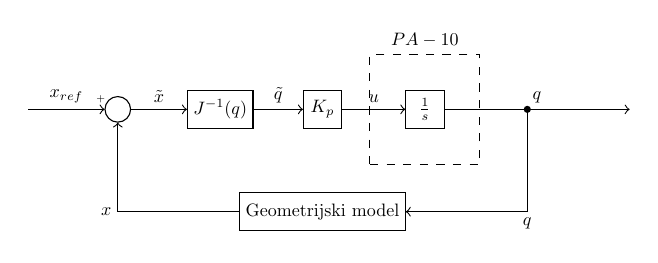
\begin{tikzpicture}[node distance=2cm,auto,=>latex',scale=0.65, every node/.style={transform shape}]
\node [input, name=input] {};
\node [sum, right of=input] (sum) {};
\node [block, right of=sum] (jac) {$J^{-1}(q)$};
\node [block, right of=jac] (k1) {$K_p$};
\node [right of=k1](pa10){};
\node [block, right of=k1] (int1) {$\frac{1}{s}$};
\node [fit = (int1)(pa10), dashed,draw,inner sep=0.45cm, label=$PA - 10$] (Box){};
\node [support, right of=int1](s1){};
\node [output, right of=s1] (output) {}; 
\node [block, below of=k1] (geom) {Geometrijski model}; 

\draw [->] (input) -- node[name = qin] {{$x_{ref}$}} node[pos=0.95] {{\tiny $+$}} (sum);
\draw [->] (sum) -- node[name = xer] {{$\tilde{x}$}} (jac);
\draw [->] (jac) -- node[name = qerr] {{$\tilde{q}$}} (k1);
\draw [->] (k1) -- node[name = u] {{$u$}} (int1);
\draw [->] (int1) -- node[name = q] {{$q$}} (output);
\draw [->](s1) |- node[name = q2] {{$q$}}(geom);
\draw [->](geom) -| node[name = x] {{$x$}}(sum);


\fill (s1) circle [radius=2pt];
\end{tikzpicture}
	\caption{Bločna shema krmiljenja referenčne lege vrha robota}
	\label{fig:xfeedback}
\end{figure}

\subsection{Admitančno vodenje} \label{sec:vodenje-admitance}

Robotski mehanizem PA-10 je industrijski robot s segmenti iz pretežno litega železa. Segmenti imajo relativno veliko maso, sklepi pa relativno visoko trenje. Lahko predpostavimo, da ima manipulator veliko lastno impedanco. Pojem mehanske impedance izvira iz analogije električne impedance. Predstavlja pa razmerje med silo (\textit{F}) in hitrostjo (\textit{v}) 

\begin{equation}
Z(s) = \frac{F}{v} = ms + b + \frac{k}{s}
\end{equation}
oziroma razmerje med silo in pozicijo (\textit{x})

\begin{equation}
Z(s) = \frac{F}{x} = ms^2 + bs + k,
\end{equation}
kjer je \textit{m} masa, \textit{b} viskozno dušenje, \textit{k} togost \cite{mihelj_hapt}.



Za doseči admitančno vodenje je potrebno še upoštevati podatek o silah in navorih, ki delujejo na vrhu robota. Na vrh robota pritrjen senzor sil in navorov JR3. Izmerjene sile in navori bodo označene s $\textbf{h}_{JR3}$, referenčne sile in navori pa z $\textbf{h}_{ref}$. Napaka sile je tako definirana kot:
\begin{equation} \label{eq:herr}
\tilde{\textbf{h}} = \textbf{h}_{ref} - \textbf{h}.
\end{equation}

Sila kot rezultat delovanja robota na okolico je odvisna od hitrosti oz. pozicije vrha robota. Premikal se bo v smeri želene sile. Zato lahko napako sile dodamo v regulator lege \ref{eq:outcontrol}. Definiramo referenčno pozicijo v odvisnosti od hitrosti

\begin{equation} \label{eq:xrefforce}
\textbf{x}_{ref} = \textbf{K}_{hP}\tilde{\textbf{h}} + \textbf{K}_{hI} \int_{0}^{t}\tilde{\textbf{h}}d\xi.
\end{equation}

Dobili smo PI regulator sile interakcije. Čeprav je bilo pri definiciji mehanske impedance definirano, da je to razmerje med silo ter hitrostjo, se raje uporablja razmerje med silo ter pozicijo. Meritve sile so podvržene šumu, integrator pa deluje kot nizkopasovni filter. Z vpeljavo integratorja, dosežemo to, da se bo robot premikal v smeri želene sile s hitrostjo $\textbf{K}_{hI} \int_{0}^{t}\tilde{\textbf{h}}d\xi$.

Z vstavitvijo enačbe \ref{eq:xrefforce} v \ref{eq:outcontrol} je mogoče zapisati celotno regulacijsko enačbo za vodenje robota v zunanjih koordinatah z upoštevanjem delovanja zunanjih sil na vrh robota.

\begin{equation} \label{eq:admitcontrol}
\textbf{u} = \textbf{K}_p  \textbf{J}^{-1}(\textbf{K}_{hP}\tilde{\textbf{h}} + \textbf{K}_{hI} \int_{0}^{t}\tilde{\textbf{h}}d\xi - \textbf{x})
\end{equation}


\section{Rezultati}

Zgrajen strežnik se je ovrednotilo z vodenjem robota v kontaktu s togo okolico. Najprej je bil opravljen preizkus na vzbujanje s stopničasto funkcijo. Primerjalo se je, odzive robota na različno velikost stopnice pri različnih vzorčnih časih, 100 Hz ter 500 Hz.

\begin{figure}[!h]
	
	   \begin{subfigure}[b]{0.5\textwidth}
	   	\includegraphics[width=\textwidth]{./slike/figure_0_hz_100dt}

	   	\caption{Odziv na stopnico pri vzorčni frekvenci 100 Hz.}
	   	\label{fig:0hzgraph100}
	   \end{subfigure}
	   ~ %add desired spacing between images, e. g. ~, \quad, \qquad, \hfill etc. 
	   %(or a blank line to force the subfigure onto a new line)
	   \begin{subfigure}[b]{0.5\textwidth}
	   	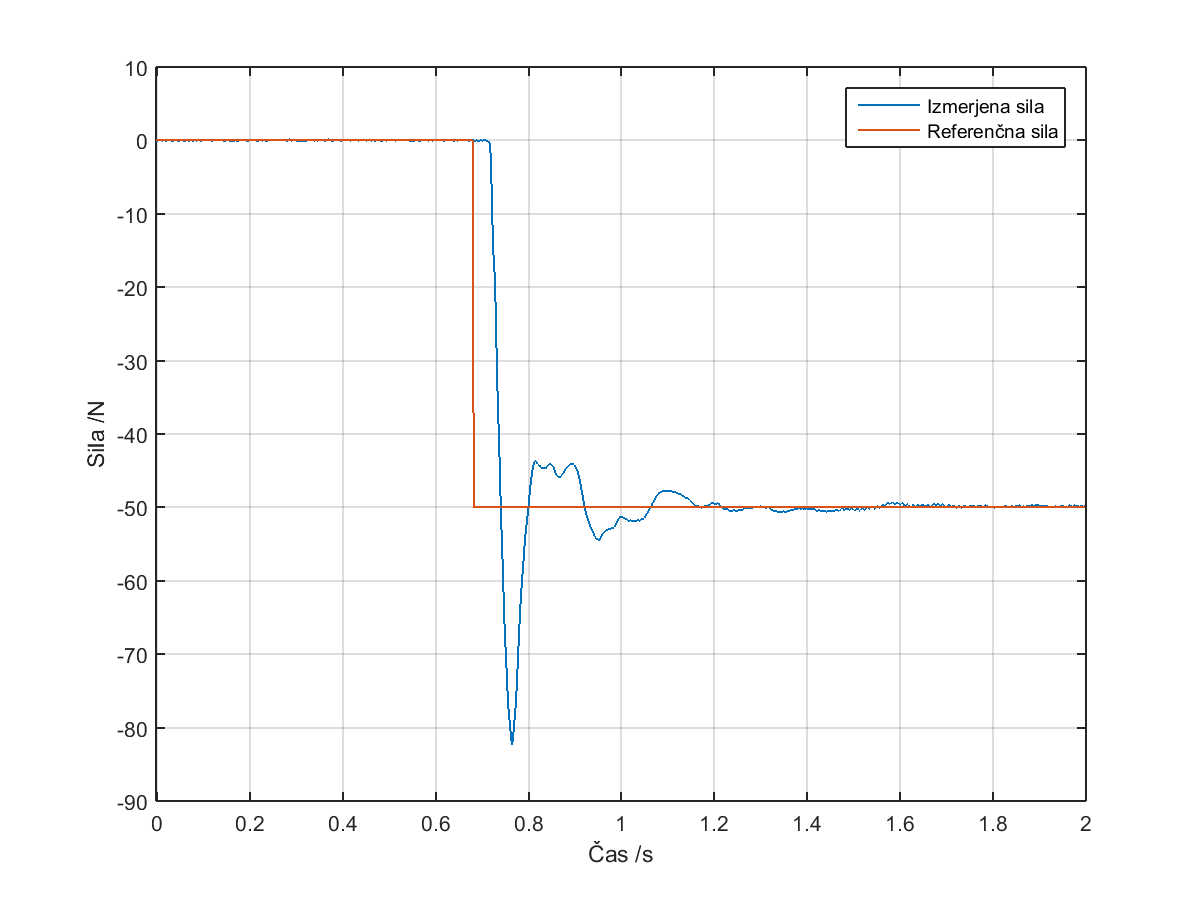
\includegraphics[width=\textwidth]{./slike/figure_0_hz_5}
	   	\caption{Odziv na stopnico pri vzorčni frekvenci 500 Hz.}
	   	\label{fig:0hzgraph500}
	   \end{subfigure}
	
\end{figure}

Nato se je ovrednotilo vodenje strežnika s 500 Hz pri referenčnem signalu sinusne oblike. Rezultate pri različnih frekvencah sinusnega signala prikazujejo sledeči grafi.

\begin{figure}[!h]
	
	\begin{subfigure}[b]{0.5\textwidth}
		\includegraphics[width=\textwidth]{./slike/figure_5_hz}
		\caption{Odziv na sinusni signal s frekvenco 0.5 Hz.}
%		\label{fig:0hzgraph100}
	\end{subfigure}

	\begin{subfigure}[b]{0.5\textwidth}
		\includegraphics[width=\textwidth]{./slike/figure_10_hz}
		\caption{Odziv na sinusni signal s frekvenco 1 Hz}
%		\label{fig:0hzgraph500}
	\end{subfigure}
	
	\begin{subfigure}[b]{0.5\textwidth}
		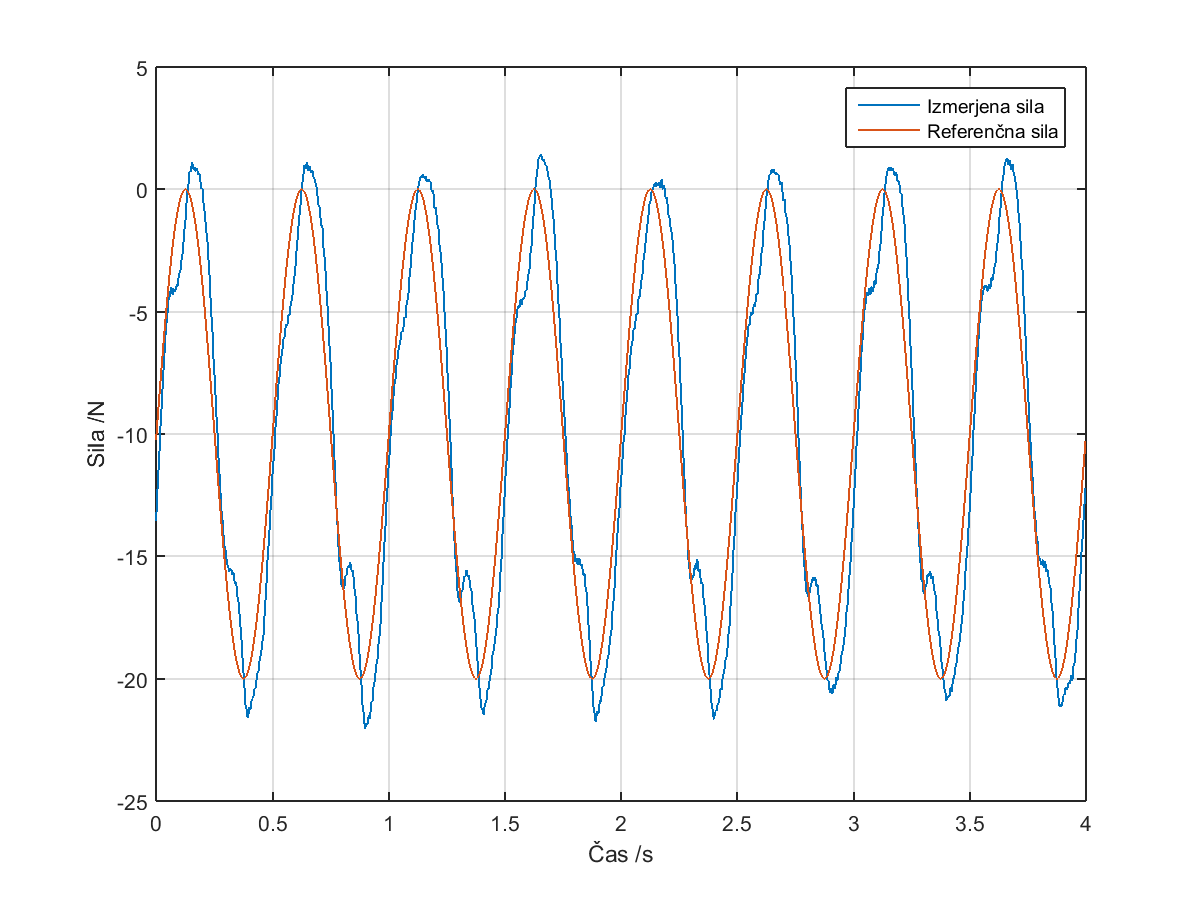
\includegraphics[width=\textwidth]{./slike/figure_20_hz}
		\caption{Odziv na sinusni signal s frekvenco 2 Hz}
%		\label{fig:0hzgraph500}
	\end{subfigure}
	
	\caption{Odzivi na sinusni signal}
				
\end{figure}

\section{Zaključek}

Vodenje robotov v kontaktu z togo okolico zahteva visoko vzorčno frekvenco. Admitančno vodenje omogoča vodenje sile vrha robota preko hitrosti v sklepih vendar je zato potrebno namestiti ustrezen senzor. Namenski strežnik, ki je bil zgrajen za vodenje robota PA-10 dosega zastavljene cilje. Hkrati pa omogoča prilagoditev na dodatne funkcije v kolikor bodo te v prihodnosti potrebne. Nadaljnje delo bo implementirati vodenje preko dinamičnega modela. 

\small

\bibliographystyle{ieeetr}
\bibliography{literatura}
%\begin{thebibliography}{1}
%
%\bibitem{ERK} ERK, http://www.ieee.si/erk/index.html 
%\bibitem{Zbornik} B. Zajc, A. Trost: Zbornik triindvajsete mednarodne Elektrotehniške in računalniške konference ERK 2014, 22. - 24. September 2014, Portorož, Slovenija
%
%
%
%\end{thebibliography}

\end{document}
